%\chapter{Introduction}



\chapter{Static analysis and Goblint}
\section{Overview}

\section{Theory} %TODO
TODO
Knaster–Tarski theorem\\
Kleene fixed-point theorem\\
monotonic function f on complete partial order L -> f has least fix-point\\
different possibilities for solving: kleene, round-robin\\
Goblint uses recursive demand-driven solver -> query system to exchange results between analyses\\
reachability analysis as an example with constraint system etc.\\

\section{Getting started}
Appendix: Setup\\
Adding an own analysis


\chapter{Verifying correct usage of file handles}
\section{Common problems using files}
The following examples for common problems served as a guideline for the implementation and contain comments starting with \verb|WARN: | that indicate where warnings would be output.

\refListing{01-ok.c} shows opening a file \verb|log.txt| and appending the line "Testing..." to it. At the end the file is closed.
\listingC{01-ok.c}{Everything fine?}

\paragraph*{fopen}
This might seem fine, since the file will be created if it doesn't exist, but what happens if the file can't be written to?
If the file exists but we don't have write access, running the code will result in a segmentation fault at \verb|fprintf|.
We forgot to check the result of \verb|fopen| which returns an error code if the file couldn't be opened successfully.
This case is handled by the implementation and can also be checked using the specification language. In this example warnings should be issued that the file handle might not be open after line 5.

A corrected version could look like \refListing{02-ok-checked.c}.
\listingC{02-ok-checked.c}{Success check for fopen}
For brevity reasons a success check is omitted in the following examples and it's assumed that the file could be opened without errors. The specification version can be easily adjusted to conform to this by just replacing a few states, whereas the manual implementation would always warn about maybe unopened file handles.

\refListing{03-no-open.c} shows what happens if the file handle was not opened before using it. When running the program, this leads to a segmentation fault.
\listingC{03-no-open.c}{Missing fopen}

\paragraph*{fclose}
Not closing files is not necessarily an error since file handles are closed at the end of the program anyway, but it's not good practice and might lead to unwanted behavior.
Imagine a program that is done writing important information to a file but doesn't close it. What happens if the program gets stuck in calculations or on user input and other programs want to use the file? See \refListing{04-user-input.c} for example. Without the call to \verb|fclose|, the written content might not be flushed until the program terminates. Running with some content in the file resulted in an empty file at the point of user input.
\listingC{04-user-input.c}{Motivation for fclose: flushing}

\refListing{05-no-close.c} has comments for warnings that would be issued. There is a warning where the file was opened and a summary of unclosed files at the end of the program.
\listingC{05-no-close.c}{Missing fclose}

\paragraph*{fprintf}
Writing to a file which is opened read-only as demonstrated in \refListing{06-open-mode.c} is another problem. Bugs of this kind might be hard to find, since this executes without errors - there is just nothing written to the file.
\listingC{06-open-mode.c}{Wrong open mode}

Other functions like \verb|fscanf, fputc, fgetc, fwrite, fread| are not analyzed, since the problems are similar to \verb|fprintf|.


\section{A domain for representing file handle usage}
Since the program behavior is merely approximated, one has to differentiate between information that may or must be true. For illustration May- and Must-Sets with their corresponding join operation and the meaning of the empty set are described below.
\begin{description}
\item[Must-Set] Property must be true for all elements, but not all elements with the property must be in the set. $\sqcap = \cap$, $\emptyset = \top$.
\item[May-Set] Property may be true or not for each element, but all elements for which  it is true must be in the set. $\sqcap = \cup$, $\emptyset = \bot$.
\end{description}
If the sets contain elements we want to warn about, then the difference concerning warnings is described below.
\begin{description}
\item[Must-Set] Precision: every warning is an error, but the program may still have errors.
\item[May-Set] Soundness: there might be false positives, but if there are no warnings, then the program is error-free.
\end{description}

Since it should be possible to track multiple file handles, a map \textbf{M} from variables (or better L-values) \textbf{K} to another domain \textbf{V} is needed. The bottom value for \textbf{M} is the empty map.
The domain \textbf{V} represents one file handle. \refListing{fileDomainType.ml} shows how its type \verb|t| is defined.
\listingML{fileDomainType.ml}{Type of the file handle domain}
\begin{description}
\item[t'] Must and May don't correspond to the sets from above but describe something different here. As long as the file handle is safely described, \verb|Must ...| is used. As soon as there might be multiple possible records, \verb|May ...| is used. There are some special cases though, which we will come to later.

\item[record] contains the variable \verb|var| that was used as a key, the location stack \verb|loc| and \verb|state|.

\item[state] can be \verb|Open(filename, mode)| or \verb|Close|.

\item[mode] can be \verb|Read| if the file is opened read-only with mode \verb|r| or \verb|Write| for all other modes.

\item[loc] is a stack of locations from the assignment to \verb|var| down to the use of the stdio-function. It is maintained as a special value inside \textbf{M}. On entering a function, the location of the call site is pushed, and popped again when leaving the function.
\end{description}
The location stack is kept because the location of the stdio-function might not always be the location where the warning should be issued. \refListing{07-location-stack.c} defines a custom function for opening files. The warnings should be placed at the call to this function instead of at the call to \verb|fopen|.
%TODO does this work correctly??
\listingC{07-location-stack.c}{Location of warning when using custom function for opening files}
However, using a normal stack could lead to infinite strictly ascending chains as shown in \refListing{08-location-stack-chain.c}. Once the uninitialized variable \verb|b| contains 0, the file will be opened. This normally happens pretty fast before overflowing the call stack. So the program runs fine, but the analysis would get stuck with an ever growing location stack. To avoid this, the location stack behaves as an ordered set, i.e. if a location is already contained in the stack, it won't be pushed. %TODO check code!
\listingC{08-location-stack-chain.c}{Infinitely growing location stack}
TODO: limitation: %TODO
\listingC{09-location-stack-alternate.c}{Mutually recursive functions and the location stack}
As mentioned above, there are some special cases concerning May-Sets:
\begin{itemize}
\item The empty set represents \textbf{V}'s bottom element: \verb|May {}| $ = \bot$
\item The set with exactly one element \verb|May {x}| means that that the record \verb|x| might not safely describe the file handle anymore because of an unsupported operation (e.g. pointer arithmetic).
\item The set with more than one element \verb|May {x, y, z ...}| contains possible alternative records. 

Even if the correct one is not known, these alternatives can be used to answer questions about the state during the analysis.

Assume for example that the set contains records with the states \verb|Open(..., Read)| and \verb|Open(..., Write)|. In this case it is safe to say that the file is opened - if it is writable on the other hand is unknown. Another example: all states are \verb|Close| but with different locations. %TODO is this ok for join? how is it done?
\end{itemize}
\refFigure{fileDomain} shows the ordering that is used.
\begin{figure}[ht]
  \centering
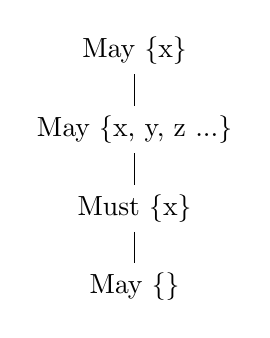
\begin{tikzpicture}[]
  \node (1) {May \{x\}};
  \node [below of=1] (2) {May \{x, y, z ...\}};
  \node [below of=2] (3) {Must \{x\}};
  \node [below of=3] (4) {May \{\}};

  \path[every node/.style={font=\sffamily\small}]
    (1) edge node {} (2)
    (2) edge node {} (3)
    (3) edge node {} (4);
\end{tikzpicture}
  \caption{Ordering of the file domain}
  \label{fig:fileDomain}
\end{figure}\\
% describe join
The join operation for \textbf{V} is the union of all records, with the exception of 1-element May-Sets which lead to the set itself. The result is always a May-Set.
%\verb|join x y = {records of x}| $\cup$ \verb|{records of y}|.\\
\begin{align*}
join(x,y)=\left\{\begin{array}{cl}
records(x), & \mbox{if }may(x) \wedge |records(x)|=1\\
records(y), & \mbox{if }may(y) \wedge |records(y)|=1\\
records(x) \cup records(y), & \mbox{else} \end{array}\right.
\end{align*}


\section{An analysis for checking file handle usage}
The analysis uses the following transfer functions, which are called by the framework. The current context is kept in \verb|ctx|, \verb| D.t| is the type of the used domain, \verb| lval| (L-value), \verb|exp| (expression), \verb|fundec| (function declaration) and \verb|varinfo| (variable) are types from CIL.
%\begin{lstlisting}[language=ML]
%let assign ctx (lval:lval) (rval:exp) : D.t = ...
%let branch ctx (exp:exp) (tv:bool) : D.t = ...
%let body ctx (f:fundec) : D.t = ...
%let return ctx (exp:exp option) (f:fundec) : D.t = ...
%let enter ctx (lval: lval option) (f:varinfo) (args:exp list) : (D.t * D.t) list = ...
%let combine ctx (lval:lval option) fexp (f:varinfo) (args:exp list) (au:D.t) : D.t = ...
%let special ctx (lval: lval option) (f:varinfo) (arglist:exp list) : D.t = ...
%\end{lstlisting}
\begin{description}
\item \inlineML{assign ctx (lval:lval) (rval:exp)}\\
Assignment of an expression \verb|rval| to a L-value \verb|lval|.\\
Warn about changed file pointer if \verb|lval| $\in$ \verb|D| and mark entry unsafe. %TODO

\item \inlineML{branch ctx (exp:exp) (tv:bool)}\\
Enter a branch where the condition \verb|exp| is either true or false, depending on \verb|tv|.\\
Used to handle error-case of \verb|fopen|. If \verb|exp| compares an L-value \verb|lval| with an integer and the expression can be transformed into \verb|lval==0| with \verb|tv| being true, then remove \verb|lval| from the domain.

\item \inlineML{body ctx (f:fundec)}\\
Called when the body of a function is entered.

\item \inlineML{return ctx (exp:exp option) (f:fundec)}\\
Called once a function returns, \verb|exp| contains the expression if one is returned.\\
If the returning function is \verb|main|, print out a summary of unclosed files if there are any.
If a L-value is returned, save it as a special entry \verb|return_var| in the domain.
Finally remove all formals and locals of the function from the domain.

\item \inlineML{enter ctx (lval: lval option) (f:varinfo) (args:exp list)}\\
Enter a function \verb|f| with arguments \verb|args| and the returned value optionally being saved to \verb|lval|.\\
Save the current location to the location stack if the function is not \verb|main|.

\item \inlineML{combine ctx (lval:lval option) fexp (f:varinfo) (args:exp list) (au:D.t)}Leave a function \verb|f| and combine the updated domain \verb|au| with the context of the call site. Counterpart to \verb|enter|.\\
Pop the top element from the location stack. If \verb|return_val| is set and there is an \verb|lval| which is assigned to, save the entry \verb|return_val| points to with \verb|lval| as a new key in the domain.


\item \inlineML{special ctx (lval: lval option) (f:varinfo) (arglist:exp list)}\\
Called for functions that are not defined in the program.\\
Add the current location to the location stack. Issue warnings and/or modify domain depending on \verb|lval| and the called function. The details are described below.
\end{description}


\section{Soundness vs. Precision}


\chapter{A general specification for regular safety properties}
%\section{Interesting types of constraints}

\section{Representing the state of properties using an automaton}


\section{Specification format}
The basic structure of the specification format is modeled after the DOT graph description language (\refListing{example.dot} would yield the graph shown in \refFigure{dot-example} (generated using \verb|dot2tex|)).
\listingML{example.dot}{A digraph using the DOT graph description language}
%\graphic[scale=.7]{dot-example}{The graph produced by \refListing{example.dot}}
\begin{figure}[ht]
  \centering
\begin{tikzpicture}[>=latex',line join=bevel,]
  \pgfsetlinewidth{1bp}
%%
\pgfsetcolor{black}
  % Edge: a -> b
  \draw [->] (61.912bp,88.824bp) .. controls (55.705bp,76.411bp) and (47.016bp,59.031bp)  .. (35.198bp,35.396bp);
  \definecolor{strokecol}{rgb}{0.0,0.0,0.0};
  \pgfsetstrokecolor{strokecol}
  \draw (71bp,62bp) node {step1()};
  % Edge: a -> c
  \draw [->] (80.606bp,89.275bp) .. controls (84.407bp,83.351bp) and (88.592bp,76.479bp)  .. (92bp,70bp) .. controls (96.149bp,62.112bp) and (100.17bp,53.273bp)  .. (107.5bp,35.839bp);
  \draw (118bp,62bp) node {step2()};
  % Node: a
\begin{scope}
  \definecolor{strokecol}{rgb}{0.0,0.0,0.0};
  \pgfsetstrokecolor{strokecol}
  \draw (70bp,106bp) ellipse (27bp and 18bp);
  \draw (70bp,106bp) node {a};
\end{scope}
  % Node: c
\begin{scope}
  \definecolor{strokecol}{rgb}{0.0,0.0,0.0};
  \pgfsetstrokecolor{strokecol}
  \draw (114bp,18bp) ellipse (42bp and 18bp);
  \draw (114bp,18bp) node {Warning};
\end{scope}
  % Node: b
\begin{scope}
  \definecolor{strokecol}{rgb}{0.0,0.0,0.0};
  \pgfsetstrokecolor{strokecol}
  \draw (27bp,18bp) ellipse (27bp and 18bp);
  \draw (27bp,18bp) node {b};
\end{scope}
%
\end{tikzpicture}
  \caption{The graph produced by \refListing{example.dot}}
  \label{fig:dot-example}
\end{figure}
A specification file contains two types of definitions: nodes and edges. The labels of nodes are output. The labels of edges are the constraints.

\begin{description}
\item[warnings]
Nodes are used to define warnings and have an implicit back edge to the previous node if they are used as a target.
Alternatively warnings can be specified like this: \verb|node1 -w1,w2,w3> node2 constraint| (\verb|w1|, \verb|w2| and \verb|w3| will be output when the transition is taken).

\item[start node]
The start node of the first transition is the start node of the automaton.

\item[end nodes]
End nodes are specified by \verb|node -> end _|.\\
\verb|_end| is the local warning for nodes that are not in an end state, \verb|_END| is the warning at return of \verb|main| (\verb|$| can be used as a placeholder for the list of keys).

\item[wildcard]
An edge with \verb|_| as a constraint matches everything.

\item[forwarding]
Edges with \verb|->>| (or \verb|-w1,w2>>| etc.) are forwarding edges, which will continue matching the same statement for the target node.\\
\end{description}
The grammar for parsing the specification is shown below in a modified Backus-Naur-Form where the symbols $*, +, ?$ are used as in regular expressions. The implementation is based on the lexer and parser generators ocamllex and ocamlyacc. \verb|<string>| can be single- or double-quoted and quotes inside a string can be escaped with \verb|\|. Single- and multi-line comments are supported and already filtered out by the lexer.
\begin{grammar}

<file> ::= <definition> EOL \verb|/* definitions are seperated by line breaks */|
\alt <definition> EOF
\alt EOL
\alt EOF

<node> ::= <word> <ws>+ <string> \verb|/* word is [_0-9a-zA-Z], ws is whitespace */|

<edge> ::= <word> <ws>* `-' (<word> (`,' <word>)*)? `>'? `>' <ws>* <word> <ws>+

<definition> ::= <node>
\alt <edge> <stmt>

<stmt> ::= <var> `=' <expr>
\alt <expr>

<key> ::= `\$' <word>

<var> ::= <key>
\alt <identifier> \verb|/* e.g. foo, _foo, _1, but not 1a */|

<regex> ::= `r' <string>

<arguments> ::= <expr>
\alt <arguments> `,' <expr>

<binop> ::= `<' \alt `>' \alt `==' \alt `!=' \alt `<=' \alt `>=' \alt `+' \alt `-' \alt `*' \alt `/'

<expr> ::= `(' <expr> `)'
\alt <regex>
\alt <string>
\alt <bool> \verb|/* true or false|
\alt <nexpr> \verb|/* omitted: numerical expressions are evaluated */|
\alt <var>
\alt <identifier> `(' <arguments> `)' \verb|/* function call */|
\alt `_' \verb|wildcard|
\alt <expr> <binop> <expr> \verb|/* omitted: numerical comparisons are evaluated */|

\end{grammar}


\section{Shortcuts for making the specification more concise}
More sane/human-readable.


\chapter{Example use cases}
%http://smallcultfollowing.com/babysteps/pubs/2013.07.17-NEU.pdf
%What Rust doesn’t have...
%– Null pointers
%– Dangling pointers
%– Segmentation faults
%– Data races
%– Mandatory GC

\section{File handles redux}

\section{Locks}
Different kinds of locks + table of functions for them.
Locks with counters not regular -> see extenstions.

\section{Heap usage: malloc and free}


\chapter{Providing a better interface}
\section{Web frontend}
Screenshots.
Online version.


\chapter{Tests and real world examples}
Test some specifications on kernel code?
Benchmarks?


\chapter{Ideas for further development}
\section{Non-regular safety properties}
E.g. locks with counters.


\chapter{Conclusion}

